The first section of this chapter gives a brief introduction to Coding Theory and its applications. Also, widely used terminologies and notations in Coding are provided. Following up, the de Bruijn sequence, an attractive combinatorial object in Coding theory, and the results surround it are presented. The universal cycles, which is the generalised version of de Bruijn sequence, are also concerned. The applications of these such sequences are surveyed and provided at the end of this chapter.

\section{Coding Theory}
% \begin{itemize}
%     \item \href{https://sci-hub.st/10.1007/s12243-021-00877-5}{A novel ofine indoor acoustic synchronization protocol: experimental analysis}: Another usage of de Bruijn sequence in synchronization.
%     \item \href{http://www-groups.mcs.st-andrews.ac.uk/~pjc/talks/21pmtia/pjc_pmtia2.pdf}{Synchronizing automata, de Bruijn graphs, and applications}:
%     \item \href{https://www4.comp.polyu.edu.hk/~comp2322/Bit\%20and\%20Frame\%20Synchronization\%20Techiques.pdf#:~:text=Synchronization\%20techniques\%20will\%20guide\%20the\%20receiving\%20system\%20in,the\%20need\%20for\%20error\%20control\%20at\%20higher\%20levels.}{Bit and Frame Synchronization
% Techniques}
% \end{itemize}
% {\color{red} A field where many application of de Bruijn sequences are found}
Transmitting, storing, protecting data (and so on) are challenging problems because of various factors: noisy channels, bandwidth, inter-symbol interference, $\ldots$. Coding theory is the study of the properties of codes and their fitness that helps dealing with these issues. In academic research, codes are involved in data-transmission, data-storage, data-compression, cryptography, error-detection and correction. 

\subsection{Brief overview}\label{subsec:brief_overview}
The article, "A Mathematical Theory of Communication" of Claude Shannnon, published in 1948, was considered to mark the birth of Coding Theory. In his work, Shannon showed that when a noisy communication channel is given, he defined a number, called the capacity of the channel, such that reliable communication can be achieved at any rate below the channel capacity, if proper encoding and decoding techniques are used. 


In more than half a century, coding theory has seen phenomenal growth. Many codes have been well-studied and have various application in real life. For example, Reed-Solomon code is used in 3G, 4G network, Turbo code is used in 5G network. Both Turbo code and LDPC code are channel coding technique that Data modems, telephone transmission, NASA Deep Space Network use to get the bit through. 

Usually, coding is divided into \textit{source coding} and \textit{channel coding}. 

Source coding plays a role of changing the message source to a code that is suitable for transmitting through the channel. For example, ASCII code is a source coding standard converting each character to a byte of 8 bits is an example of source coding. Another way to think about source coding is to treat it as a compress-decompress process. At the transmitter, the source encoder compresses the message for the purpose of economizing on the length of the transmission. At the other end, the source decoder decompresses the received signal or sequence. The commonly used compression algorithms include Huffman code used in JPEG, MPEG, MP3 files, Lempel-Ziv code used in ZIP files,$\cdots$.

Because of physical and engineering limitations, channels are not ideal: their output may differ from their input because of noise or manufacturing defects. The transmitted message may become distorted and the receiver might not realize that the message was corrupted. Additionally, there are applications, such as magnetic and optical mass storage media, where certain patterns are not allowed to appear in the channel's bit stream. The main role of channel coding is to overcome such limitations by encoding the message again after the source coding while maintaining the channel as transparent as possible from the source and destination points of view. 

\begin{figure}
    \centering
    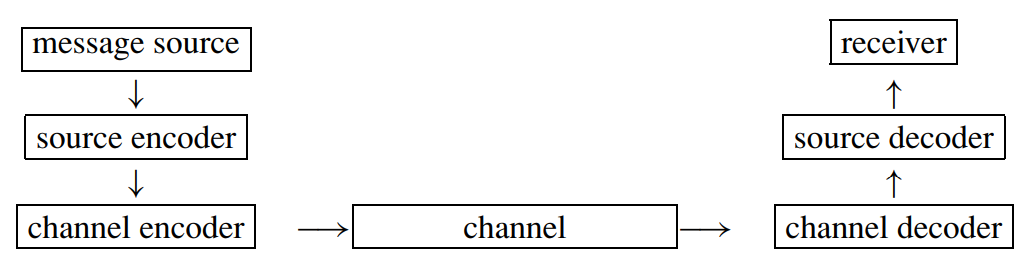
\includegraphics[scale=0.5]{fig/sourceandchannelcoding.png}
    \caption{Model of source and channel coding~\cite{ling2004coding}.}
    \label{fig:sourcechannelcoding}
\end{figure}

Section~\ref{subsec:brief_overview} has introduced to basic idea of coding theory. In the next section, this thesis provides the commonly used notations and terminologies of this research field.
\subsection{Notation and terminologies}
The most essential element of coding theory is \textbf{codeword}, which is a sequence of code symbols taken from a code alphabet
\begin{definition}[Code Alphabet]
    A code alphabet is set $\Sigma=\left\{a_{1},a_{2},\ldots,a_{q}\right\}$ of size $q$. The elements of $\Sigma$ are called code symbols, letters, and bits if $q=2$. A $q$-ary word of length $n$ over $\Sigma$ is a sequence (or string) $\bfw=w_{1}w_{2}\ldots w_{n}\in\Sigma^{n}$ with each $w_{i}\in\Sigma$ for all $i$. 
\end{definition}
In practice, the size of a code alphabet is often the size of a finite field, which is the power of a prime number. Hence, for simplicity, $\Sigma$ can be treated as a set of the first $q$ non negative integers without ambiguity. More particularly, the notation $\Sigma={0,1,2,\ldots,q-1}$ can be used instead.
\begin{definition}[Code and Codeword]
    A $q$-ary block code $C$ over $\Sigma$ is a nonempty set $C$ of $q-ary$ words of the same length $n$. Each element of $C$ is called a codeword in $C$.
\end{definition}
The study of a code $C$ involves the following process in an example of channel coding. Suppose that $\Sigma$ and $\Sigma^{\prime}$ are finite input and output of the channel respectively. Let $\bfm$, taken out of $M$ possible information words, be a message input to the channel encoder. Through a desired channel encoder, the message $\bfm$ is mapped to a longer codeword $\bfc\in\Sigma^{n}$. The word $\bfc$ is transmitted through the channel, become $\bfy\in\Sigma^{\prime n}$. After receiving $\bfy$, the role of the channel decoder is to produce codeword $\hat{\bfc}$ and a decoded information word $\hat{\bfu}$, aiming to have $\bfc=\hat{\bfc}$ and $\bfu=\hat{\bfu}$. Consequently, the mapping at the channel encoder needs to be one-to-one, and the size of the code $C$ is the maximal possible number of messages, or $\card{C}=M$.

Observe that, using code $C$, it takes a sequence of length $n$ to encode a sequence of length $\log_{\card{\Sigma}}(\card{C})$. In other words, $n-\log_{\card{\Sigma}}(\card{C})$ "redundant" bits were added to the message so that the channel can achieve its goal. Accordingly, a quantity concerning this redundancy was introduced, called \textit{(information) rate}. 
\begin{definition}[Information rate]\label{def:information_rate}
    The (information) rate of a code $C$ over an alphabet of size $q$ is defined as:
    \begin{align}
        R_{C}= \dfrac{\log_{q}(\card{C})}{n}.
    \end{align}
\end{definition}

Works in coding theory, including this thesis, are interested in designing codes with high rate, along with its efficient encoder, decoder, that can be used in specific situations. 

Based on their motive or their intrinsic properties, codes are categorized into linear codes, constrained codes, error-correcting codes, error-detecting codes,$\ldots$. This thesis focus on the combination of a constrained code, run length limited, and positioning code. A brief introduction to constrained code is given in the next section.

\subsection{Constrained code}\label{subsec:constrained_code}
Constrained Code is a sub-field of Coding theory, studies to design codes satisfying given constrained. The inspiration for the research of constrained codes comes from real problems. The transmitted data needs to follow some given standards which are necessary for the code to surmount the flaw of the environment. For instance, in the CD disc storage, errors tend to occur when there is a sequence of many consecutive $0$ bits. Consequently, it's crucial to construct codes that should avoid a long sequence of $0$ bits. A famous code invented to overcome this challenge is \gls{RLL} code by Immink~\cite{immink1990runlength}. \gls{RLL} codes are defined by $2$ parameters: $d, k$, and denoted by $(d,k)$-RLL, where $d$ and $k$ are two non-negative integers such that $d\leq k$. A finite length binary sequence 
is said to satisfy the $(d,k)$-RLL constraint if its number of $0$'s between $2$ consecutive $1$ bits is at least $d$ and at most $k$.

Illustration is a convenient way to begin understanding things. In constrained code, a graph, usually called labeled graph, is a helpful visualization technique. More particularly, a labeled graph is a directed graph with its vertices and edges labeled. Vertices in labeled graph are also called states. And the start and end vertices of a directed edge are called initial and terminal states respectively. Given a state $v$, in-edges of $v$ are edges treating $v$ as terminate state. Similarly, out-edges of $v$ are edges taking $v$ as initial state. 

For example, the graph in figure~\ref{fig:d_k_RLL} represents a $(d,k)$-RLL code. It can be verified that a sequence $w$ satisfies the $(d,k)$-RLL constraint if and only if a path whose edge labeling is $w$ exists in the graph.

\begin{figure}[htbp]
    \centering
    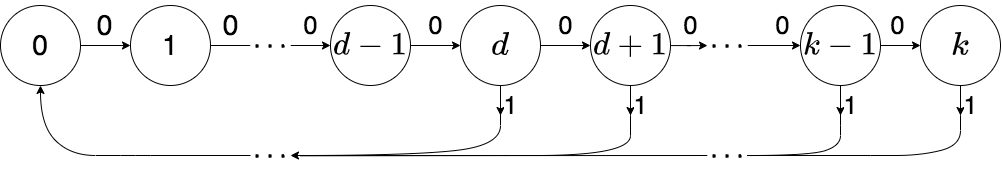
\includegraphics[scale=0.4]{fig/RLL.png}
    \caption{Graph representation of $(d,k)$-RLL code.}
    \label{fig:d_k_RLL}
\end{figure}

Labeled graphs are however more than just visualization tools. Using finite state splitting algorithm, they become encoders. In a constrained system, a very common problem is designing an encoding algorithm, which maps arbitrary user sequences into sequences obeying the constraints. Nevertheless, it's crucial to note that there are many kinds of encoders, depending on their objectives. For instance, there are encoders not taking any sequences as input, their goal are just to generate sequences satisfying given constraints. Such encoders are focused in this thesis. 

Beside constrained code, another combinatorial object drawing many attentions in coding theory is positioning code, also known by the name de Bruijn code. The formal definition of this code and its important results are presented in the next section.

% {\color{blue}
% \begin{itemize}
%     \item What is coding (def + sth from Ling San's book)
%     \item Application of coding
%     \item What are interested element in Coding (combinatorial object, encoder, decoder)
%     \item Constrained Code (Graph presentation (remember to mention in-edge, in-coming edge), Ronny)
%     \item Notation and Terminology
% \end{itemize}
% Something about error correcting, decoding ...
% }





\section{De Bruijn Sequence}
A de Bruijn sequence (of order $k$), sometimes called a positioning sequence, over an alphabet $\Sigma$, is a sequence of symbols of $\Sigma$ such that all subsequences over $\Sigma$ of length $k$ appear exactly once. This section first explains how to use a graph to represent de Bruijn sequences, and then introduces methods to generate or decode such sequences. Important results on the granddaddy, one of the most interesting de Bruijn sequences, which play a significant role in this work, are also given. 

\subsection{Graph presentation of de Bruijn sequences}

Since the first time introduced in 1946 by de Bruijn himself, the de Bruijn graph and its related sequences have been well-studied and generalized under numerous names, including positioning sequences, m-sequences, shift register sequences \cite{song2021robust,etzion1984algorithms,fredricksen1982survey,lempel1970homomorphism,cohn1977fast}. The goal of de Bruijn was to find a recursive algorithm to enumerate the number of cyclic binary sequences of length $2^k$ such that each binary $k$-tuple appears as a window of length $k$ exactly once in each sequence. 

The first results in the de Bruijn graph focused on the alphabet of size $2$. Later, in 1951, van Aardenne-Ehrenfest and de Bruijn \cite{van1951circuits} generalized the enumeration result for any arbitrary alphabet of finite size $q$, using a generalized graph for an alphabet $\Sigma$ of size $q$. 

\begin{definition}[de Bruijn graph]
    Formally, the de Bruijn Graph of order $k$, $G_{k}$ is a directed graph with $q^{k-1}$ vertices, each one is represented by a word of length $k-1$ over an alphabet $\Sigma$ with $q$ letters. A directed edge from the vertex $\bfx=(x_{0},x_{1},\ldots,x_{k-2})$ to the vertex $\bfy=(y_{1},y_{2},\ldots,y_{k-1})$, represented by the symbol $x_{k}$, where $x_{i},y_{i}\in\Sigma$, if and only if $x_{i}=y_{i}$ for all $1\leq i\leq k-2$. We call this edge $x_{k}$ the out-edge of $\bfx$, and the in-edge of $\bfy$. Progressively, the in-degree and out-degree of a vertex $\bfx$ are the numbers of in-edges and out-edges of $\bfx$ respectively.
\end{definition}  Deduced from the definition, the in-degree and out-degree of each vertex are $q$. Thus, a de Bruijn graph is an Eulerian graph. Figure \ref{fig:dB4} gives an illustration for the graph $G_{4}$.

\begin{figure}[htbp]
    \centering
    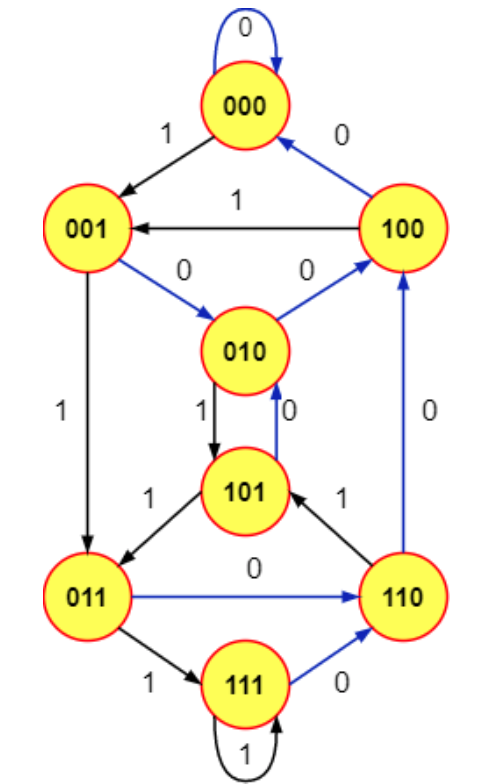
\includegraphics[scale=.3]{fig/dB4.png}
    \caption{de Bruijn graph of order $4$, $G_{4}$.}
    \label{fig:dB4}
\end{figure}

\textbf{Path}: A \textit{path} in the graph is a sequence of edges: $e_{0},e_{1},\ldots,e_{n}$ such that the terminal vertex of edge $e_{i}$ is the the initial vertex of edge $e_{i+1}$ for all $0\leq i\leq n-1$. A \textit{simple path} is a path going through each edge at most one time. Each longest simple path in a de Bruijn graph is an Eulerian cycle. A sequence formed by concatenating the symbol of each edge in the longest simple path in $G_{k}$ is called a (cyclic) de Bruijn sequence of order $k$. All the strings of length $k$ appear exactly once in each such de Bruijn sequence. The acyclic version of the de Bruijn sequence can be obtained by prepending the sequence representing the first vertex in the corresponding Eulerian cycle to the cyclic one. 

\begin{example}
    Consider an Eulerian cycle starting at vertex $000$, then the symbols representing the following edges $0,1,0,1,0,0,1,1,1,0,1,1,0,0,0$ form a de Bruijn sequence order $4$. Adding $000$ to its beginning results in an acylic one: $$0,0,0,0,1,0,1,0,0,1,1,1,0,1,1,0,0,0$$.
\end{example} 

The number of longest simple path in $G_{k}$, and also the number of de Bruijn sequences, have been proved in~\cite{van1951circuits} to be $\dfrac{q!^{q^{k-1}}}{q^{k}}$.
\begin{example}
    For $q=2,\ k=4$, there are $16$ distinct de Bruijn sequences. From figure \ref{fig:dB4}, those de Bruijn sequences are found and listed as follows:   
    \begin{center}
        \begin{tabular}{c c}
            $0000100110101111$ & $0000100111101011$ \\
            $0000101001101111$ & $0000101001111011$ \\
            $0000101100111101$ & $0000101101001111$ \\
            $0000101111001101$ & $0000101111010011$ \\
            $0000110010111101$ & $0000110100101111$ \\
            $0000110101111001$ & $0000110111100101$ \\
            $0000111100101101$ & $0000111101001011$ \\
            $0000111101011001$ & $0000111101100101$ \\
        \end{tabular}
    \end{center}
\end{example}




\subsection{Encode and decode de Bruijn sequences}
Encoding de Bruijn sequences concerns generating an arbitrary de Bruijn sequence or a de Bruijn sequence satisfying some given constraints. Finding a de Bruijn sequence is equivalent to seeking an Eulerian cycle in a de Bruijn graph. In~\cite{fleury1883deux,hierholzer1873moglichkeit}, efficient algorithms to find Eulerian cycles are presented. Especially, the approach in~\cite{fleury1883deux} can be used to generate all binary de Bruijn sequences. However, since the graph must be stored, applying such algorithms to find a positioning sequence requires exponential $O(q^k)$ space.

Besides the graph-based approach, there are other well-known methods to construct such sequences, including \gls{lfsr}, recursive methods, greedy methods, and concatenation approaches.

The idea of \gls{lfsr} is to design a feedback function $f$ mapping length $k$ strings to $\left\{0,1\right\}$. Starting with an initial length $k$ string, $f$ is repeatedly applied to the last $k$ symbols of the current string to generate the next symbol until the maximal length of a de Bruijn sequence is reached. If $f$ is linear, then, the function $F(\alpha)= \alpha f(\alpha)$ is said to be a \gls{lfsr}, where $\alpha$ is a length $k$ string. \gls{lfsr}s based on primitive polynomials generate maximal length sequences (positioning sequences) having length $2^{k}-1$ that miss only the all $0$ string. The downside of this method is that it's compulsory to find a primitive polynomial first.

De Bruijn sequences can also be constructed via recursion by applying Lempel's $D$-morphism $D:\{0,1\}^{m}\to\{0,1\}^{m-1}$ which maps a string $\alpha = \alpha_{1}\alpha_{2}\ldots\alpha_{m}$ to $\beta = \beta_{1}\beta_{2}\ldots\beta_{m-1}$, where each $b_{i} = a_{i} + a_{i+1}\ (mod\ 2)$. Nevertheless, an exponential amount of space is also required by these recursive strategies. 

Surprisingly, greedy approaches are also able to generate de Bruijn sequences. The greedy construction starts with a seed string, then repeatedly applies some greedy rule to determine the next symbol of a sequence. The algorithm stops when it is impossible to add another symbol without creating a duplicate substring of length $k$, or some termination condition is reached. The different explicit greedy rules result in different implementation greedy algorithms~\cite{martin1934problem,alhakim2010simple,fredricksen1982survey,alhakim2021revisiting}. Such constructions, however, have a major drawback: they require exponential space.

Despite many constructions being known, and even a useful survey has been given by Fredricksen~\cite{fredricksen1982survey}, things are not quite the same for the decoding problem. This problem, discovering the position within a particular sequence of any specified $k$-tuple, has been much less well studied. There are just some classical de Bruijn sequences with sub-linear decoding algorithm~\cite{mitchell1996method,tuliani2001bruijn,kociumaka2016efficient}. 

\subsection{Results on lexicographically minimal de Bruijn sequence}

The lexicographically minimal de Bruijn sequence, or \textbf{granddaddy sequence} as called by Knuth~\cite{knuth2013art}, is one the most interesting among other de Bruijn sequences. An example of granddaddy is provided in example~\ref{exp:granddaddy}.
\begin{example}[Granddaddy of order $6$]\label{exp:granddaddy}
    \[0000001000011000101000111001001011001101001111010101110110111111\]    
\end{example}
Both efficient encoder and decoder of this sequence have been found.

The encoding algorithm is actually a concatenation scheme, which is later called \gls{fkm} algorithm, the abbreviation of Fredrickesen, Kessller, and Maiorana, who discovered this strategy~\cite{fredricksen1978necklaces,fredricksen1986algorithm}. Its complexity has been proved to be constant amortized time per symbol by Frank Ruskey et.al~\cite{ruskey1992generating} in 1992.

Though its construction and the related algorithm has been found in 1978, about 40 years ago, the granddaddy's decoder has just been discovered recently in 2016 by Kociumaka, Radoszewski, and W. Rytter~\cite{kociumaka2016efficient}. Denote $\bfx$ as a granddaddy sequence of order $k$, and $v$ is a length $k$ arbitrary substring. Then the decoding algorithm, denoted by $\cD_{KRR}$, returns $\cD_{KRR}(v)$ being the one and only position of $v$ in the whole sequence $\bfx$. Kociumala et.al also proved that $\cD_{KRR}$ works in $O(k^2\log(q))$-time in the word-RAM model and $O(k^{2})$-time in unit-cost RAM model.

\section{Universal Cycles}\label{sec:universal_cycles}
A more general way to look at de Bruijn sequences is the universal cycle ($U$-cycle). 
\begin{definition}[Universal cycle]
    Given a finite set $\mathcal{T}_{k}$ of distinct of combinatorial objects of "rank $k$", an $U$-cycle of $\mathcal{T}_{k}$ is a cyclic sequence $\cU=(a_0,a_1,\ldots,a_n)$ such that $(a_{i+1},\ldots,a_{i+k})$, $0\leq i\leq n$, run through each element of $\mathcal{T}_{k}$, where index addition is performed modulo $n$.
\end{definition} 
An order $k$ binary de Bruijn sequence is eventually an $U$-cycle of the set of all length $k$ binary strings. The studies of $U$-cycle are concerned with the existence and construction of $U$-cycles for many combinatorial objects such as strings, permutations, partitions, subsets, multisets, lattice paths, vector spaces weak orders, etc~\cite{chung1992universal,horan2013universal,jackson2009research,johnson2009universal,hurlbert2009universal,jackson2009recursive}. Section~\ref{subsect:fanchung} provides results for permutations, partitions, and subsets of a set of $n$ distinct symbols, where $n$ is a positive integer. These results were first summarized by \citeauthor{chung1992universal} in~\cite{chung1992universal}.
%, for example: the set of all $n!$ permutations of $\left\{1,2,\ldots,n\right\}$, partitions of $\left\{1,2,\ldots,n\right\}$~\cite{chung1992universal}. 

\subsection{Permutations, partitions and subsets of \texorpdfstring{$n$}{n} distinct symbols}\label{subsect:fanchung}
Consider the set $S_{n}$ of all $n!$ permutations of $\left\{1,2,\ldots,n\right\}$. With each value of $n$, set $S_{n}$ may not always contain any $U$-cycles, such as $n=3$. All $6$ permutations of $\left\{1,2,3\right\}$ are $S_{3}=\left\{123,132,213,231,312,321\right\}$, and the longest cycle in $S_{3}$ one can travel is of length $4$, for instance,  $123\rightarrow231\rightarrow312\rightarrow123$, which still lacks $132, 321$. 

However, if order-isomorphism is allowed instead of requiring exact matches, $U$-cycles of $S_{n}$ exists. More precisely, an $U$-cycle $U_{n}=(a_{0},a_{1},\ldots,a_{n!-1})$, $a_{i}\in\left\{1,2,\ldots,N\right\}$, for $S_{n}$ is $n!$-tuple such that each element of $S_{n}$ is order-isomorphic to exactly one block $(a_{i+1},\ldots,a_{i+n})$, where $a_{i}=a_{j\equiv i(\mod n!)}$. Here, two $n$-tuples $\bfa=\left(a_{1},a_{2},\ldots,a_{n}\right)$ and $\bfb=\left(b_{1},b_{2},\ldots,b_{n}\right)$ are called order-isomorphic, written as $\bfa\sim\bfb$, if $a_{i}<a_{j} \Leftrightarrow b_{i}<b_{j}$ for all $0<i,j\leq n$. An example of $U$-cycle for $S_{3}$ is :
\[1\ 4\ 5\ 2\ 4 \ 3\]

By order-isomorphism, each $3$-tuple in the above $U$-cycles can be mapped into elements of $S_{3}$ as follow:
\begin{align*}
    145\sim123 \\
    452\sim231 \\
    524\sim312 \\
    243\sim132 \\
    431\sim312 \\
    314\sim213 
\end{align*}
and hence, the equivalent cycle is $123\rightarrow 231\rightarrow 312\rightarrow132\rightarrow312\rightarrow 213\rightarrow123 $. The construction of de Bruijn graphs can be imitated to construct the transition graph for $S_{n}$. Each permutation plays the role of a vertex. Their suffix of length $n-1$ is analyzed to establish its edges to other permutations. Takes the vertex $231$ of $S_{3}$ as an example. From its suffix $31$, one can go to $312$. But since order-isomorphism is accepted, and note that $31\sim21\sim32$, there are also edges connecting $231$ to $213$ and $321$. The whole transition graph of $S_{3}$ is shown in figure \ref{fig:S3_graph}.

\begin{figure}[htbp]
    \centering
    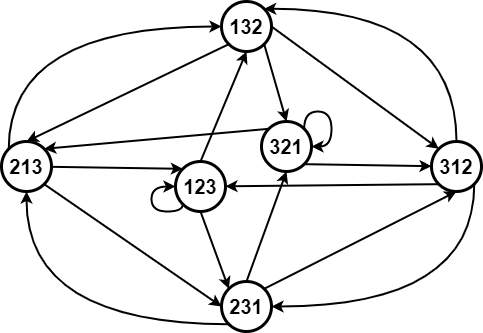
\includegraphics[scale=0.5]{fig/PermutationGraph.png}
    \caption{Transition graph of $S_{3}$.}
    \label{fig:S3_graph}
\end{figure}

It is proved that the transition graph of $S_{n}$ is Hamiltonian, and a Hamiltonian cycle in the transition graph corresponds to an $U$-cycle in $S_{n}$. Now, the key question is how to represent a $U$-cycle of an Hamiltonian cycle, like the sequence $1\ 4\ 5\ 2\ 4\ 3$ represents $123\rightarrow 231\rightarrow 312\rightarrow132\rightarrow312\rightarrow 213\rightarrow123 $. Even with $S_{3}$, is $5$ the smallest number of distinct symbols necessary for an $U$-cycle. More generally, how many distinct symbols does an $U$-cycle of $S_{n}$ use at least? 

Actually, in $S_{3}$, one can do better with $4$ symbols. For example, the sequence $1\ 4\ 2\ 3\ 4\ 2$ is the representation of a Hamiltonian cycle:
\[132\rightarrow312\rightarrow123\rightarrow231\rightarrow321\rightarrow213\rightarrow132\]

The following sequence is an example with $5$ symbols for $S_{4}$:
\[1\ 2\ 3\ 4\ 1\ 2\ 5\ 3\ 4\ 1\ 5\ 3\ 2\ 1\ 4\ 5\ 3\ 2\ 4\ 1\ 3\ 2\ 5\ 4 \]

Let $N(n)$ be the minimum number required for an $U$-cycle of $S_{n}$, it is proved that:
\[N(2)=2,\ N(3) = 4,\ N(4)=5\ \mathrm{and}\ n+1\leq N(n)\leq 6n\ \mathrm{for}\ n\geq5\]

Fan Chung believes that the equation happens at $n+1$. However, their belief remains an unsolved conjecture until now.
\begin{conjecture}
    $N(n)=n+1$.
\end{conjecture}

Constructing transition graph is also help finding $U$-cycle for the set of $P_{n}$ of partitions of the set $\left\{1,2,\ldots,n\right\}$. The partitions can be represented by sequence of length $n$ $(a_{0},a_{1},\ldots,a_{n})$, where $a_{i}=a_{j}$ indicates the $i$-th element and $j$-th element are in the same group of the partition. The transition graph of $P_{n}$ is illustrated in figure~\ref{fig:P3_graph}.

\begin{figure}[htbp]
    \centering
    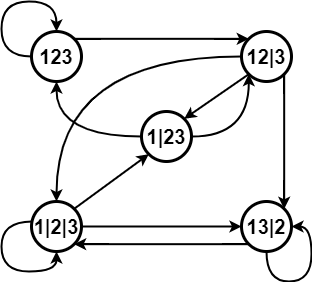
\includegraphics[scale=0.5]{fig/partitions.png}
    \caption{Transition graph of $P_{3}$.}
    \label{fig:P3_graph}
\end{figure}

The transition graph of $P_{n}$ is proved to be Hamiltonian by showing that it can be clustered to be an Eulerian graph. 

It is more challenging to study the family ${n \brack k}$ of all $k$-element subsets of a set of $n$ distinct elements $\left\{0,1,\ldots,n-1\right\}$. This thesis provides an example of an $U$-cycle for the case $n=5,k=2$:
\[1\ 3\ 2\ 5\ 4\ 2\ 1\ 5\ 3\ 4\]

The question about the condition for the existence of the universal cycle for such a family is still not answered completely. The difficulty here is that a transition graph for ${n \brack k}$ isn't able to be defined explicitly. This issue is caused by the distinguishing feature of an $k$-set. More precisely, a $k$-element subset might occur in any $k!$ possible order in the $U$-cycle, but it is only allowed to occur once. Fan Chung and Graham made a conjecture on this problem and the first person who can solve it would earn a prize awarded by the author's conjecture.

\begin{conjecture}[Fan Chung's conjecture]\label{conjecture:fanchung}
    Universal cycle for ${n \brack k}$ always exists provided $k$ divides $\dbinom{n-1}{k-1}$ and $n$ is large enough.
\end{conjecture}

It's easy to see that conjecture~\ref{conjecture:fanchung} is true for $k=1,2$. Effort on this question has just cracked completely the cases $k=3,4,5$ (with some aid of a computer), and $k=6$ whenever $n\ \mathrm{and}\ k$ are relatively prime(~\cite{hurlbert1994universal,jackson1993universal}). For $k\geq 7$, and $k=6$ when $n\ \mathrm{and}\ k$ are not relatively prime, conjecture~\ref{conjecture:fanchung} remains open. 

Besides studying the existence of $U$-cycle on different kinds of sets, designing algorithms that create universal cycles is also concerned.
\subsection{Universal cycles algorithms for other classes of sets}
There are researches focusing on using generalized the \gls{fkm} algorithm and greedy algorithm to create universal cycles for a class of sets. Moreno proved that this method works for the set of rotations of the lexicographically largest $i$ necklace~\cite{moreno2004theorem}. The aperiodic strings in the set of all $k$-ary strings of length $n$ can be generated the same way as shown by Au in~\cite{au2015generalized}. All these results are later generalized by Joe Sawada et.al in~\cite{sawada2016generalizing}. More particularly, let $\bfS$ be the set of length $n$ $k$-ary strings such that the following closure conditions are obeyed:
\begin{itemize}
    \item The set of strings $\bfS$ is closed under rotation.
    \item Its subset of necklaces is closed under replacing any suffix of length $i$ by $k^i$. 
\end{itemize}

Then, the greedy and \gls{fkm} algorithm create the lexicographically smallest universal cycle of $\bfS$. Several such classes $\bfS$ are listed in example~\ref{exp:closed_S}.

\begin{example}\label{exp:closed_S}
Recall that $\Sigma_{q}=\{1,2,3,\ldots,q\}$ is a code alphabet of size $q$, and $\Sigma_{q}^{n}$ is the set of $q$-ary sequences of length $n$ over alphabet $\Sigma$. The following sets satisfy the closure conditions for the existence of universal cycles proved by Sawada~\cite{sawada2016generalizing}.
\begin{itemize}
    \item \textbf{Minimum Sum}: $\bfS\in\Sigma_{q}^{n}$ is a set of length $n$ strings with sum over all of its symbol at least $s$, where $s$ is a given constant.
    \item \textbf{Frequency of $q$}: $\bfS\in\Sigma_{q}^{n}$ contains the strings with at least $l_{q}$ copies of $q$, where $l_{q}$ is a given constant.
    \item \textbf{Frequency of $i<q$}: $\bfS\in\Sigma_{q}^{n}$ contains the strings with at most $u_{i}$ copies of $i<q$. Here, $u_{i}$ is a given constant.
    \item \textbf{Avoiding a substring}: $\bfS\in\Sigma_{q}^{n}$ contains the strings that do not contain a given pattern $\alpha\in\Sigma_{q-1}^{m}$, for some $m\geq1$, as a cyclic substring. 
    \item \textbf{Union and Intersection}: Let $\bfS_{1}$ and $\bfS_{2}$ be $2$ set obeying the closure conditions, then both $\bfS_{1}\cup \bfS_{2}$ and $\bfS_{1}\cap \bfS_{2}$ also satisfy those conditions.
\end{itemize}
\end{example}
Note that, in example~\ref{exp:closed_S}, the union and intersection of the proper sets $\bfS$ allow to combine the previous results to create more interesting classes of sets that have universal cycles. 

Section~\ref{sec:universal_cycles} has provides different research directions and results on the universal cycle, which is a generalization of de Bruijn sequences. The applications of de Bruijn sequences and their generalizations will be presented in the next section. 


\section{Applications }
The reason why de Bruijn graph, its sequence, and their generalizations are having so much attention is due to their diverse important applications. Very soon after the formal definition of this graph was given birth, one of its first applications was found in the introduction of shift-register sequences in general and linear feed-back registers in particular~\cite{golomb19821967}. Throught out the years, these type of sequences and graphs have found a variety of applications.

In cryptography, for example, the Baltimore Hilton Inn used de Bruijn sequence to install a cipher lock system for each of its rooms in lieu of the conventional key-lock system~\cite{fredricksen1982survey}. The low-cost n-stage shift register was used to generate maximum-length pseudorandom sequences in stream cipher, though later, this method was proved to be vulnerable to known-plaintext attack~\cite{lempel1979cryptology}.

De Bruijn sequences also opened a new field of research surround its complexity. Agnes Hui Chan et.al studied the complexity and the distribution of the complexities of de Bruijn sequences~\cite{chan1982complexities}. Especially, for binary sequence with period $2^n$, they come up with a fast algorithm determining its complexity~\cite{games1983fast}. Edwin on himself analysed the structure and complexity of nonlinear binary sequence generators~\cite{key1976analysis}. Tuvi et.al studied the error linear complexity spectrum of binary sequences with period $2n$~\cite{etzion2009properties}. Also Tuvi, in his joint work with Lampel~\cite{etzion1984construction}, found a construction of de Bruijn sequence to show that the lower bound of its complexity ($2^{n-1}+n$) is attainable for all $n$.

In~\cite{lempel1985design}, A.Lampel and M.Cohn are interested in designing an universal test sequeces for VLSI (very large scale integration chip). A binary sequence is called $(s,t)$-universal, $s>t$, if when shifted through a register of length $s$, it exercises every subset of $t$ register positions. Their proposed method was concatenating a set of de Bruijn sequences of appropriate length. In~\cite{barzilai1983exhaustive}, Zeev Barzilai .et.al also demonstrated an application of de Bruijn sequence in VLSI self-testing.

There are also other applications requiring two-dimensional version of de Bruijn sequeces. And the research about two-dimensional generalization of de Bruijn sequences comes to call. One well-known version is called pseudo-random arrays. In 1976, Mac Williams and Neil Sloane~\cite{macwilliams1976pseudo} gave a simple description of pseudo-random arrays and studied several of their nice properties. In 1988, Tuvi~\cite{etzion1988constructions}, represented a new version of pseudo-random arrays to construct perfect maps. Another approach by Bruck Stein~\cite{bruckstein2012simple}, he combined a de Bruijn sequence and a half de Bruijn sequece to study it robust and self-location properties. Studies~\cite{hsieh2001decoding,morano1998structured,pages2005optimised,salvi2010state,van1994digital} used pseudo-random arrays to with applications to robust undetectable digital watermarking of two-dimensional test images, and structured light. 

More surprisingly, de Bruijn's modern applications are even combined with biology, like the genome assembly as part of DNA sequencing. For example, Chaisson et.al~\cite{chaisson2009novo} described a new tool, EULER-USR, for assembling mate-paired short reads and use it to analyze the question of whether the read length matters. Compeau et.al~\cite{compeau2011apply} represented a method using de Bruijn graph to genome assembly. In 2001, Pevzner et.al~\cite{pevzner2001new} abandoned the classical “overlap - layout - consensus” approach in favor of a new Eulerian Superpath approach, that, for the first time, resolves the problem of repeats in fragment assembly. Later on, in 2003, Yu Zhang and Michael Waterman~\cite{zhang2003eulerian}, adapted the Pevzner's method to global multiple aligment for DNA sequences. In DNA storage, Han Mao et.al~\cite{chang2017rates,kiah2016codes} studied codes and their rates for DNA sequence profiles. Their studies were based on de Brujn graph.

In some new memory technologies, mainly in racetrack memories, and other ones which can be viewed as an $l$-read channel, synchronization errors (which are shift errors known also as deletions and sticky insertions) occur. By proposing a new de Bruijn based schema, used locally-constrained de Bruijn sequence to construct such code, Chee et.al~\cite{chee2021locally} are able to increase the rate of codes which correct the synchronization errors. Locally-constrained de Bruijn sequences and codes (sets of sequences) are of interest in their own right from both practical and theoretical points of view.

Recently, in 2021, a novel application of de Bruijn sequence has been found in quantum communication. Generally, to transmit quantum information between a satellite and the ground station, a timing and synchronization system has been used. Having observed that the intrinsic properties of positioning sequence are very suitable for this system, Peide Zhang et.al~\cite{zhang2021timing} have modulated it into \gls{HdB} sequence to transmit along the quantum channel. %More details about this application are provided and clarified in the following chapter, chapter~\ref{chapter:motivation}.




% Lưu ý: Mẫu ĐATN này được thiết kế phù hợp với đồ án tốt nghiệp theo hướng nghiên cứu. Mẫu đề tài này là gợi ý tham khảo. Tuỳ từng đề tài, cấu trúc có thể thay đổi ít nhiều. Sinh viên cần tham khảo ý kiến của giáo viên hướng dẫn để đưa ra cấu trúc hợp lý nhất cho đề tài của mình. 

% Trước khi viết ĐATN, sinh viên cần đọc kỹ hướng dẫn và quy định chi tiết về cách viết ĐATN trong Phụ lục A. 

% Khi đóng quyển ĐATN, sinh viên cần lưu ý tuân thủ hướng dẫn ở phụ lục A.9

% SV cần đặc biệt lưu ý cách hành văn. Mỗi đoạn văn không được quá dài và cần có ý tứ rõ ràng, bao gồm duy nhất một ý chính và các ý phân tích bổ trợ để làm rõ hơn ý chính. Các câu văn trong đoạn phải đầy đủ chủ ngữ vị ngữ, cùng hướng đến chủ đề chung. Câu sau phải liên kết với câu trước, đoạn sau liên kết với đoạn trước. Trong văn phong khoa học, sinh viên không được dùng từ trong văn nói, không dùng các từ phóng đại, thái quá, các từ thiếu khách quan, thiên về cảm xúc, về quan điểm cá nhân như “tuyệt vời”, “cực hay”, “cực kỳ hữu ích”, v.v. Các câu văn cần được tối ưu hóa, đảm bảo rất khó để thể thêm hoặc bớt đi được dù chỉ một từ. Cách diễn đạt cần ngắn gọn, súc tích, không dài dòng.


% Chương 1 có độ dài từ 3 đến 6 trang với các nội dung sau đây


% \section{Problem Statement}
% \label{sec:dvd}
% Phần này sinh viên mô tả bài toán cần giải quyết, lý do tại sao lại chọn bài toán đó, ý nghĩa/tầm quan trọng của bài toán.

% Tiêu đề của chương này có thể để là ``đặt vấn đề'', hoặc lấy chính tên của bài toán mà sinh viên định giải quyết, ví dụ có thể đặt tiêu đề là ``Bài toán dự đoán …” 


% \section{Background and Problems of Research} 
% \label{sec:giaiphap}
% Sinh viên trước tiên cần trình bày tổng quan các kết quả của các nghiên cứu hiện nay cho bài toán giới thiệu ở phần \ref{sec:dvd}. Sau đấy, sinh viên đưa ra các hạn chế của các giải pháp hiện tại. 

% \section{Research Objectives and Conceptual Framework}
% Trong chương này, sinh viên trước hết trình bày mục tiêu của đồ án là gì, sau đấy sinh viên đề xuất định hướng giải pháp của mình. Tốt nhất là với trình bày từng giải pháp đối với mỗi vấn đề nêu ra trong chương \ref{sec:giaiphap}. 

% \section{Contributions}
% Trong phần này sinh viên liệt kê cụ thể, ngắn gọn các đóng góp của đồ án. Ví dụ: 

% Đồ án này có 3 đóng góp chính như sau:

% \begin{enumerate}
% \item Đồ án đề xuất một phương pháp tiền xử lý dữ liệu nhằm loại bỏ nhiễu và dữ liệu ngoại lai trước khi đưa vào huấn luyện mô hình.
% \item \ldots
% \item \ldots 
% \end{enumerate}

% \section{Organization of Thesis}
% Phần còn lại của báo cáo đồ án tốt nghiệp này được tổ chức như sau. 

% Chương 2 trình bày về v.v. 

% Trong Chương 3, em/tôi giới thiệu về v.v.

% Chú ý: Sinh viên cần viết mô tả thành đoạn văn đầy đủ về nội dung chương. Tuyệt đối không viết ý hay gạch đầu dòng. Chương 1 không cần mô tả trong phần này. 

% Ví dụ tham khảo mô tả chương trong phần bố cục đồ án tốt nghiệp: Chương *** trình bày đóng góp chính của đồ án, đó là một nền tảng ABC cho phép khai phá và tích hợp nhiều nguồn dữ liệu, trong đó mỗi nguồn dữ liệu lại có định dạng đặc thù riêng. Nền tảng ABC được phát triển dựa trên khái niệm DEF, là các module ngữ nghĩa trợ giúp người dùng tìm kiếm, tích hợp và hiển thị trực quan dữ liệu theo mô hình cộng tác và mô hình phân tán.  

% Chú ý: Trong phần nội dung chính, mỗi chương của đồ án nên có phần Tổng quan và Kết chương. Hai phần này đều có định dạng văn bản “Normal”, sinh viên không cần tạo định dạng riêng, ví dụ như không in đậm/in nghiêng, không đóng khung, v.v... 

% Trong phần Tổng quan của chương N, sinh viên nên có sự liên kết với chương N-1 rồi trình bày sơ qua lý do có mặt của chương N và sự cần thiết của chương này trong đồ án. Sau đó giới thiệu những vấn đề sẽ trình bày trong chương này là gì, trong các đề mục lớn nào.

% Ví dụ về phần Tổng quan: Chương 3 đã thảo luận về nguồn gốc ra đời, cơ sở lý thuyết và các nhiệm vụ chính của bài toán tích hợp dữ liệu. Chương 4 này sẽ trình bày chi tiết các công cụ tích hợp dữ liệu theo hướng tiếp cận “mashup”. Với mục đích và phạm vi của đề tài, sáu nhóm công cụ tích hợp dữ liệu chính được trình bày bao gồm: (i) nhóm công cụ ABC trong phần 4.1, (ii) nhóm công cụ DEF trong phần 4.2, nhóm công cụ GHK trong phần 4.3, v.v...

% Trong phần Kết chương, sinh viên đưa ra một số kết luận quan trọng của chương. Những vấn đề mở ra trong Tổng quan cần được tóm tắt lại nội dung và cách giải quyết/thực hiện như thế nào. Sinh viên lưu ý không viết Kết chương giống hệt Tổng quan. Sau khi đọc phần Kết chương, người đọc sẽ nắm được sơ bộ nội dung và giải pháp cho các vấn đề đã trình bày trong chương. Trong Kết chương, Sinh viên nên có thêm câu liên kết tới chương tiếp theo.

% Ví dụ về phần Kết chương: Chương này đã phân tích chi tiết sáu nhóm công cụ tích hợp dữ liệu. Nhóm công cụ ABC và DEF thích hợp với những bài toán tích hợp dữ liệu phạm vi nhỏ. Trong khi đó, nhóm công cụ GHK lại chứng tỏ thế mạnh của mình với những bài toán cần độ chính xác cao, v.v. Từ kết quả nghiên cứu và phân tích về sáu nhóm công cụ tích hợp dữ liệu này, tôi đã thực hiện phát triển phần mềm tự động bóc tách và tích hợp dữ liệu sử dụng nhóm công cụ GHK. Phần này được trình bày trong chương tiếp theo – Chương 5.
